\documentclass{article}

\usepackage[UTF8]{ctex}

\usepackage{changepage}

\usepackage{xspace}

\usepackage{booktabs}

\usepackage{floatrow}
% Table float box with bottom caption, box width adjusted to content
\newfloatcommand{capbtabbox}{table}[][\FBwidth]

\usepackage{blindtext}

\graphicspath{{fig/}}

\newcommand{\MATLAB}{\textsc{Matlab}\xspace}


\usepackage{listings}
\usepackage{color} %red, green, blue, yellow, cyan, magenta, black, white
\definecolor{mygreen}{RGB}{28,172,0} % color values Red, Green, Blue
\definecolor{mylilas}{RGB}{170,55,241}
\lstset{language=Matlab,%
	%basicstyle=\color{red},
	breaklines=true,%
	morekeywords={matlab2tikz},
	keywordstyle=\color{blue},%
	morekeywords=[2]{1}, keywordstyle=[2]{\color{black}},
	identifierstyle=\color{black},%
	stringstyle=\color{mylilas},
	commentstyle=\color{mygreen},%
	showstringspaces=false,%without this there will be a symbol in the places where there is a space
	numbers=left,%
	numberstyle={\tiny \color{black}},% size of the numbers
	numbersep=9pt, % this defines how far the numbers are from the text
	emph=[1]{for,end,break},emphstyle=[1]\color{red}, %some words to emphasise
	%emph=[2]{word1,word2}, emphstyle=[2]{style},    
}

\begin{document}
	
	\begin{titlepage}
		\centering
		\makebox[\textwidth][c]{
\includegraphics[width=1.1\textwidth]{cover}}
	\end{titlepage}

	\section{实验原理}

该部分主要阐明实验所采用的一些方法,主要针对数据的处理,最终训练模型从而实现预测功能。

\subsection{傅里叶变换}

傅立叶变换是一种分析信号的方法,它可分析信号的成分,也可用这些成分合成信号。
$f(t)$是$t$的周期函数,如果$t$满足以下条件:在一个以$2T$为周期内$f(t)$连续或只有有限个第一类间断点,
且$f(t)$单调或可划分成有限个单调区间,则$f(t)$以$2T$为周期的傅里叶级数收敛,
和函数$F(\omega)$也是以$2T$为周期的周期函数,且在这些间断点上函数是有限值;在一个周期内具有有限个极值点;绝对可积。
下列公式即称为积分运算$f(t)$的傅立叶变换:

\begin{figure}[ht]
	\centering
	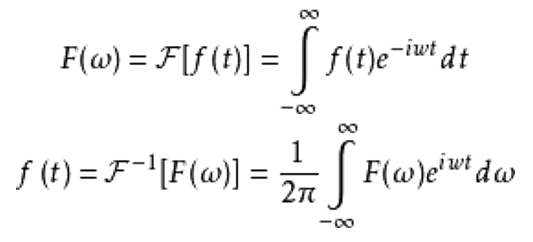
\includegraphics[width=.6\linewidth]{fft}
	\caption{连续函数傅里叶变换}
	\label{fig:fft}
\end{figure}

$f(t)$式的积分运算叫做$F(\omega)$的傅立叶逆变换。$F(\omega)$叫做$f(t)$的像函数,
$f(t)$叫做$F(\omega)$的像原函数。$F(\omega)$是$f(t)$的像。$f(t)$是$F(\omega)$原像。

由于采样值为离散数据,故而该实验采用的是离散傅里叶变换。离散傅里叶变换(DFT),
是傅里叶变换在时域和频域上都呈现离散的形式,将时域信号的采样变换为在离散时间傅里叶变换(DTFT)频域的采样。
在实际应用中通常采用快速傅里叶变换以高效计算DFT。

\begin{figure}[ht]
	\centering
	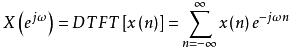
\includegraphics[width=.6\linewidth]{dtft}
	\caption{离散时间傅里叶变换}
	\label{fig:dtft}
\end{figure}

简言之,傅里叶变化就是将基于时域的特征转换成基于频域的特征。
而离散傅里叶变换就是在其基础上对离散数据基于时间进行傅里叶变换。

\subsection{主成分分析PCA}

从下图不难看出,主成分分析是将原来的变量重新组合成一组新的互相无关的变量,
同时根据实际需要从中可以取出几个较少的变量尽可能多地反映原来变量的信息的统计方法。

\begin{figure}[ht]
	\centering
	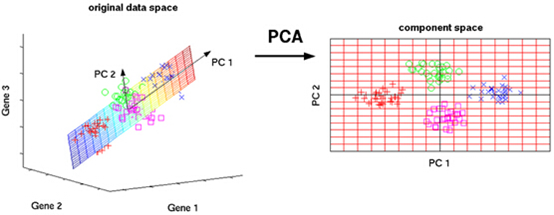
\includegraphics[width=.9\linewidth]{pca}
	\caption{主成分分析原理}
	\label{fig:pca}
\end{figure}

主成分分析能降低所研究的数据空间的维数。即用研究$m$维的$Y$空间代替$p$维的$X$空间$(m<p)$,
而低维的$Y$空间代替高维的$X$空间所损失的信息很少。

\subsection{人工神经网络的基本思想}

根据对自然神经系统构造和机理的认识,神经系统是由大量的神经细胞构成的复杂的网络,
人们对这一网络建立一定的数学模型和算法,设法使它能够实现诸如基于数据的模式识别、
函数映射等带有“智能”的功能。

\subsubsection{全连接神经网络}

对$n-1$层和$n$层而言,$n-1$层的任意一个节点,都和第$n$层所有节点有连接。
即第n层的每个节点在进行计算的时候,激活函数的输入是$n-1$层所有节点的加权。

全连接是较好的神经网络模式,但是网络很大的时候,训练速度会很慢。
部分连接就是人为切断某两个节点直接的连接,这样训练时计算量将大为减小。

\subsubsection{BP神经网络}

单个感知器能够解决线性可分的问题,但是也只能解决所谓一阶谓词逻辑问题。
所以提出了多层模型:前一层神经元的输出是后一层神经元的输入,最后一层只有一个神经元,
它接收来自前一层的$n$个输入,给出作为决策的一个输出。
	\section{实验函数}

该部分主要阐明实验过程中调用\MATLAB 平台的相关函数及使用原理。

\subsection{feedforwardnet(hiddenSizes, trainFcn)}

网络包含一系列的层次,第一层与网络输入连接,接下来的层次与上一次连接。
最后一层产生网络的输出。\texttt{feedforward}网络可以用作输入和输出的映射,
只含有一个隐含层的神经网络可以拟合任意有限的输入输出映射问题。
输入的变量有两个可以选择,前者是对隐层的设置,可以有多层并且设置每层的神经元个数。
后者可以设置训练函数,默认为\texttt{trainlm}。

\begin{table}[ht]
	\centering
	\caption{feedforwardnet函数参数说明}
	\label{tab:fwfunc}
	\begin{tabular}{ll}
		\hline
		hiddenSizes & \begin{tabular}[c]{@{}l@{}}Row vector of one or\\ more hidden layer sizes (default = 10)\end{tabular} \\ \hline
		trainFcn    & \begin{tabular}[c]{@{}l@{}}Training function\\ (default = 'trainlm')\end{tabular}                     \\ \hline
	\end{tabular}
\end{table}

\subsection{性能函数(performance function)}

Mean-Square Error( MSE) 均方误差是反映估计量与被估计量之间差异程度的度量;
Sum of Squares for Error(SSE)是误差项平方和;
Mean Squared Error with Regularization performance function(MSEREG)是正则化性能函数均方误差。

\subsection{Matlab自带神经网络库中可用的训练函数}

\begin{table}[ht]
	\centering
	\caption{训练函数参数说明}
	\label{tab:train}
	\begin{tabular}{@{}ll@{}}
		\toprule
		训练方法                  & 训练函数     \\ \midrule
		梯度下降法                 & traingd  \\
		有动量的梯度下降法             & traingdm \\
		自适应lr梯度下降法            & traingda \\
		自适应lr动量梯度下降法          & traingdx \\
		弹性梯度下降法               & trainrp  \\
		Fletcher-Reeves共轭梯度法  & traincgf \\
		Ploak-Ribiere共轭梯度法    & traincgp \\
		Powell-Beale共轭梯度法     & traincgb \\
		量化共轭梯度法               & trainscg \\
		拟牛顿算法                 & trainbfg \\
		一步正割算法                & trainoss \\
		Levenberg-Marquardt13 & trainlm  \\ \bottomrule
	\end{tabular}
\end{table}

\subsection{BP网络常用传递函数}

Log-sigmoid型函数的输入值可取任意值,输出值在0和1之间;

tan-sigmod型传递函数tansig的输入值可取任意值,输出值在-1到+1之间;

purelin线性传递函数的输入与输出值可取任意值。

BP网络通常有一个或多个隐层,该层中的神经元均采用sigmoid型传递函数,
输出层的神经元则采用线性传递函数,整个网络的输出可以取任意值。

	\section{实验背景}

根据脑电波活动为特征可以将睡眠分为四个阶段。

第一阶段:开始进入睡眠模式。此时脑波是$\alpha$波。进入第一阶段后期,脑波变成了3.5到7.5赫兹之间的$\theta$波。

第二阶段:这个阶段的脑波很不规则,会出现叫K-复合波的低幅EEG波。

第三阶段:这一阶段我们发出高幅波(3.5赫兹)、$\delta$活动的EEG信号。

第四阶段:这一阶段出现更多的$\theta$波干扰了正常的$\delta$波。人的眼睛开始快速地来回动,称作快速眼动(REM)。
	\section{实验数据}

旧数据:20个人的脑电波波形数据, 19个人的数据作为训练集, 最后一个人的数据作为测试集。
数据为mat文件, 标签为txt文件。每1000个数据对应一个标签, 例如5768000维数据对应5768维标签。

新数据:40个人的脑电波波形数据,39个人的数据作为训练集,最后一个人的数据作训练模型的预测。
数据为mat文件,每3000个数据对应一个标签,所以每个人的数据都是$3001*n$的矩阵。

	\section{实验过程}

该部分主要呈现实验的具体流程,介绍实验使用的基本方法与基本工具,并且阐明个中细节,展示主要解决的几个问题。

\subsection{训练数据提取与处理}

\begin{figure}[ht]
	\centering
	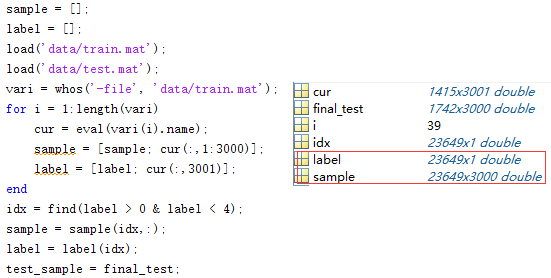
\includegraphics[width=.8\linewidth]{readin}
	\caption{读入数据}
	\label{fig:readin}
\end{figure}

首先将39个人的所有数据合并,然后过滤掉第四和第五周期的数据。继而将标签与特征数据分离,易于后期进行训练。

最终将数据分成两部分,一部分是训练特征,另一部分是标签。此外还有一个最终测试样本,但是不包含标签。

\subsubsection{三类训练样本的比例对比}

为了更直观的呈现新给的样本集合中每一类样本所占有的比例,以明确后续训练过程中的细节,
我组尝试将三类样本占总样本的比例算出,可知,第一类样本占有11.68\%,
第二类占有74.2\%,第三类占有14.00\%,由于第二类样本较多,另外两类的样本显然较少,
这也是我组在进行后续优化所要考虑的问题。

\begin{figure}[ht]
	\centering
	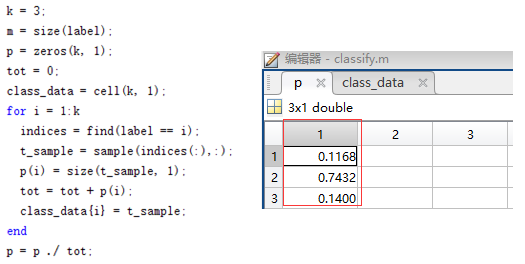
\includegraphics[width=.8\linewidth]{portion}
	\caption{各个睡眠阶段的比例}
	\label{fig:portion}
\end{figure}

\subsection{进行DTFT变换}

正如前文所述,利用计算机的FFT变换,将原本样本的时域特征变换成基于频域的特征。
在完成FFT变换后,我组绘制出三类样本所分别对应的平均FFT示意图。
进行对图片的观察后,我们得出了一系列可供参考的信息。

\subsubsection{观察频谱分布}

首先观察低频部分(见图~\ref{fig:lowf}):

\begin{figure}[ht]
	\centering
	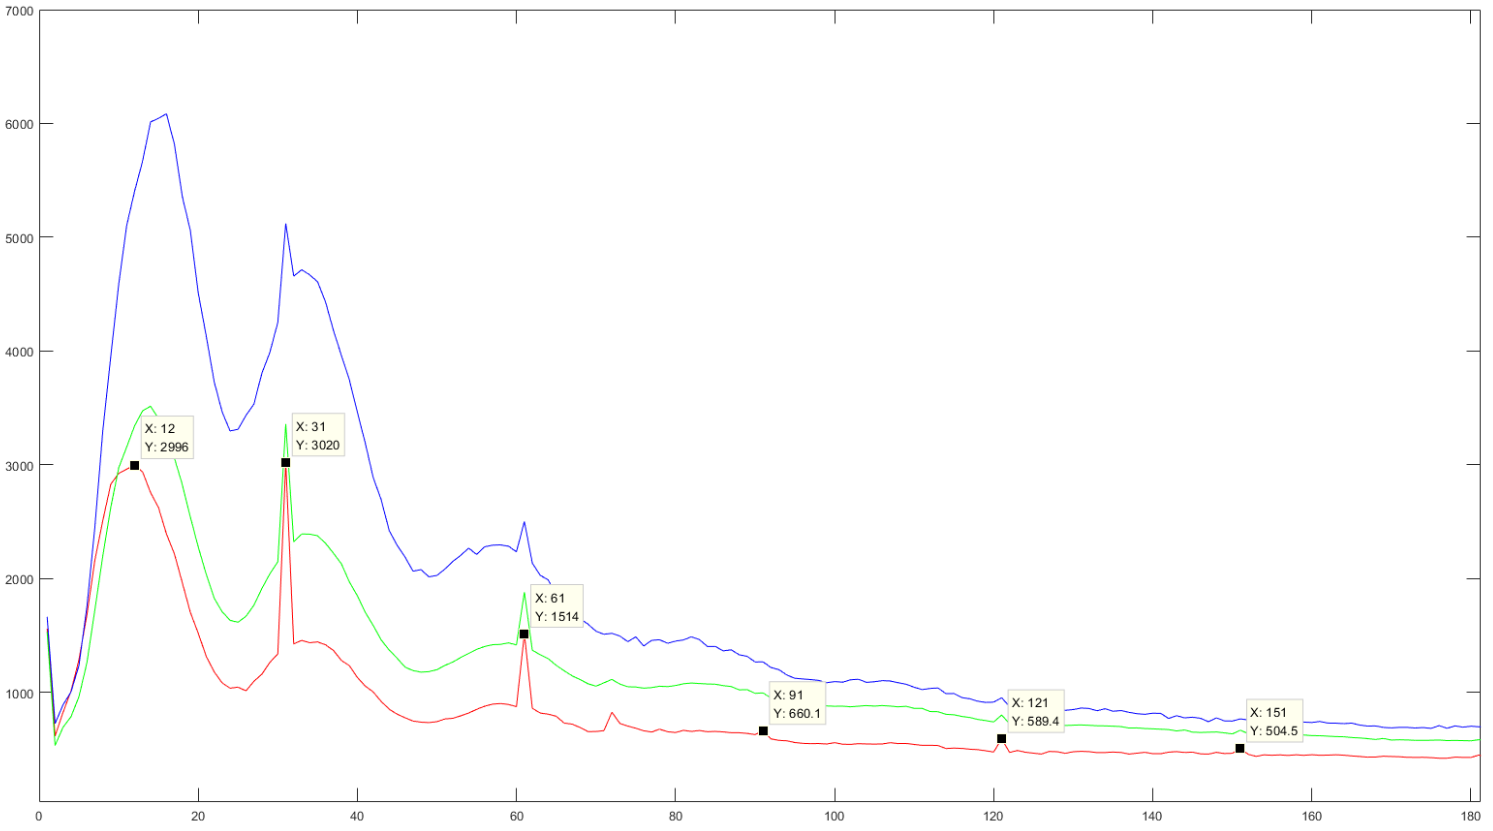
\includegraphics[width=.8\linewidth]{lowf}
	\caption{低频部分频谱分布}
	\label{fig:lowf}
\end{figure}

从上图我们可以清晰地看出在[1, 20]、[25, 40]、[50, 70]这几个频域有三个峰而且不相互重叠,
所以这几个频域能较好地表征原信号。

通过观察还可以发现,每30个频率点会出现一个异常高的尖峰,这个尖峰与其周围频谱分布极其不符,
同时每隔30个频率出现,所以我们考虑这些采样点的成分是原信号中的某种噪声或者异常偏差。
基于以上分析,我们移除这几个异常值后再进行后续处理中。

再观察高频部分(见图~\ref{fig:fivep}):

\begin{figure}[ht]
	\centering
	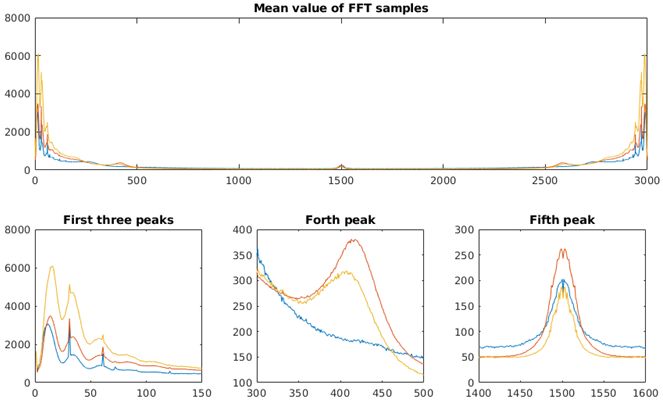
\includegraphics[width=.9\linewidth]{fivep}
	\caption{全频谱分布}
	\label{fig:fivep}
\end{figure}

在[350, 480]、 [1450, 1550]这两个频域还有比较明显的峰。

所以我们最后选取[1, 20]、[25, 40]、[50, 70]、[350, 480]、 [1450, 1550]这五个频段作为特征
进行后续处理。

\subsubsection{消除抖动}

由于单个样本的FFT曲线抖动较为剧烈,所以本文使用中值滤波对频谱分布做平滑处理。
事实上,中值滤波是一种基于排序统计理论的,能有效抑制噪声的非线性信号处理技术。
其原理在于把数字序列中一点的值用该点的一个邻域中各点值的中值代替,
让周围的值接近的真实值,从而消除孤立的噪声点。

\MATLAB 提供了非常便捷的中值滤波接口:\lstinline| medfilt1(fft_sample);|将\\
\lstinline|fft_sample|中每一列的每个值替换为这个值和上下相邻两行值得平均值。

\subsubsection{提取主频}

5.2.1小结介绍了选取频谱中的五个峰,这五个峰包含了原信号中的绝大部分的成分。
进一步观察,每个睡眠阶段在这五个峰的幅值都不尽相同,所以考虑将这五个频域中的最大值选出来,
作为五个特征。

以上所述三个操作的实现如下:

\begin{lstlisting}[language=Matlab]
function [res] = process(sample)
	ff_sample = abs(fft(sample, 3000, 2));
	% 5 peak: [1, 20], [25, 40], [50, 70], [350, 480], [1450, 1550]
	p1 = 1:20;
	p2 = [25:30, 32:40];
	p3 = [50:60, 62:70];
	p4 = 350:480;
	p5 = 1450:1550;
	sam = medfilt1(fft_sample')';	% 中值滤波
	mx1 = max(sam(:, p1), [], 2);
	mx2 = max(sam(:, p2), [], 2);
	mx3 = max(sam(:, p3), [], 2);
	mx4 = max(sam(:, p4), [], 2);
	mx5 = max(sam(:, p5), [], 2);
	comp = [1:20, [25:30, 32:40], [50:60, 62:70], 350:480, 1450:1550];
	fft_sample = fft_sample(:,comp);
	res = [fft_sample, mx1, mx2, mx3, mx4, mx5];
end
\end{lstlisting}

\subsection{数据正则化}

本实验在进行主成分分析前,对各个特征做标准正态化(normalize)。
因为PCA算法选择每个分量的时候,都尽量使得投影其上的数据尽量分散,
所以如果有个维度的数据过于分散,PCA在选取投影向量的时候就会偏向于选取该特征所在的分量,
从而丢失了较多其他维度的信息。事实上,我们得到的样本数据都是多个维度的,
即一个样本是用多个特征来表征的。但是,这些特征的量纲和数值的量级不一定一样。
如果直接使用原始的数据值,那么他们对预测目标的影响程度将是不一样的。
而通过标准化处理,可以使得不同的特征具有相同的尺度。这样,在使用梯度下降法学习参数的时候,
不同特征对参数的影响程度就一样了。

为了解决上述问题,我组将特征数据进行均值为0、方差为1的正态分布转换(见图~\ref{fig:norm})。

\begin{figure}[ht]
	\centering
	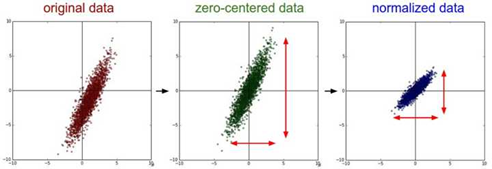
\includegraphics[width=.8\linewidth]{norm}
	\caption{数据正则化}
	\label{fig:norm}
\end{figure}

\subsection{PCA处理}

进过之前提取主要主要频率成分的操作,考虑进一步降低特征的维度。
利用PCA对正则化后的fft样本进行降维,经过试验,当选取6个主成分的时候,
已经能保留原数据中80\%以上的分布信息,训练结果也达到最好。

\begin{lstlisting}[language=Matlab]
[vec, pca_param] = pca_vec(fft_sample, 6, 1);
norm_sample = pca_trans(process(sample), vec, pca_param);
norm_tsample = pca_trans(process(tsample), vec, pca_param);
\end{lstlisting}

\subsection{移出异常值}

经过观察,特征值得分布近似符合正态分布,于是考虑将偏离均值3个标准差以上的数据
视作异常数据剔除。

\begin{lstlisting}[language=Matlab]
function [fil_sam, fil_lab, param] = rm_outlier(sample, label, param)
	m = size(sample, 1);
	idx = [];
	for i=1:m
		if sum(abs(sample(i,:) - param.mu) > 3 * param.std) == 0
			idx = [idx i];
		end
	end
	fil_sam = sample(idx,:);
	fil_lab = label(idx,:);
end
\end{lstlisting}

\subsection{数据归一化处理}

本实验为采用数据归一化,我组认为在神经网络训练中也有必要进行数据归一。

数据归一化,就是将数据映射到[0,1]或[-1,1]区间或更小的区间,比如(0.1,0.9),需要将训练和测试数据进行归一化的原因如下:

\begin{enumerate}
	\item 输入数据的单位不一样,有些数据的范围可能特别大,导致的结果是神经网络收敛慢、训练时间长。
	\item 数据范围大的输入在模式分类中的作用可能会偏大,而数据范围小的输入作用就可能会偏小。
	\item 由于神经网络输出层的激活函数的值域是有限制的,因此需要将网络训练的目标数据映射到激活函数的值域。
	例如神经网络的输出层若采用S形激活函数,由于S形函数的值域限制在(0,1),也就是说神经网络的输出只能限制在(0,1),
	所以训练数据的输出就要归一化到[0,1]区间。
	\item S形激活函数在(0,1)区间以外区域很平缓,区分度太小。例如S形函数$f(X)$在参数a=1时,$f(100)$与$f(5)$只相差0.0067。
\end{enumerate}

\subsection{创建神经网络进行训练}

\begin{figure}[ht]
	\centering
	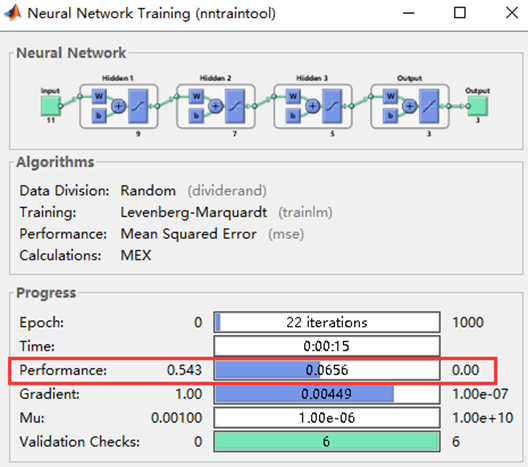
\includegraphics[width=.8\linewidth]{nnet}
	\caption{神经网络训练结果}
	\label{fig:nnet}
\end{figure}

本实验采用feedforwardnet创建训练网络,该网络结构为五层网络,出去输入层和输出层,
还有中间三层隐层。从下图中可以看出输入层为11维,即所选出的6维主成分及5维傅里叶变换主频。
中间层分别为9维、7维、5维,通过原本11维的特征,依次递减,既能有效地保持数据特征,又能逐渐收敛,得到结果输出。
	\section{实验结果}

\subsection{性能收敛}

下图所示为训练过程示意图,从下图可以看出在进行16次迭代时,通过MEX性能函数已能看出在不断的训练中,
性能达到0.071.不难看出该网络模型的收敛速度较快。

\begin{figure}[ht]
	\centering
	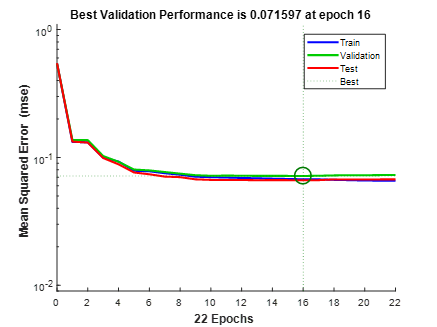
\includegraphics[width=.6\linewidth]{performance}
	\caption{神经网络训练结果}
	\label{fig:performance}
\end{figure}

\subsection{正确率87.5+\%}

\begin{figure}
	\begin{floatrow}
	\ffigbox{%
		\centering
		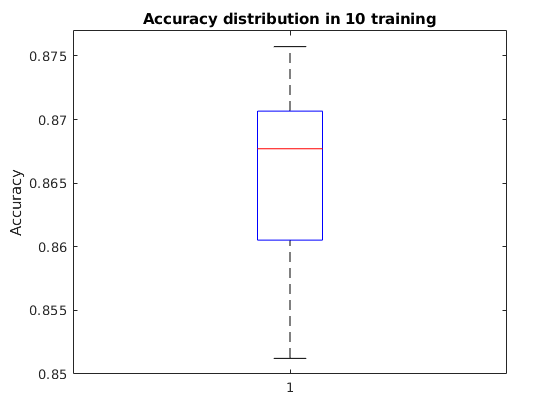
\includegraphics[width=.9\linewidth]{acc}
		\label{fig:acc}
	}{%
		\caption{10次预测正确率分布}
	}
	\capbtabbox{%
		\centering
		\begin{tabular}{cccc}
			& label 1 & label 2 & label 3 \\
			pred 1 & 95      & 32      & 1       \\
			pred 2 & 40      & 832     & 45      \\
			pred 3 & 1       & 28      & 109    
		\end{tabular}
		\label{tab:eva}
	}{%
		\caption{预测分布矩阵}
	}
	\end{floatrow}
\end{figure}

我组通过多次训练,对网络参数进行修改,并且多次重新调整训练数据的维度和数量之后,
可以将训练模型的准确率基本稳定在86+\%(见下图),并且最佳模型高达87.57\%(见下表)。
	\section{总结}

本次实验,我组采用傅里叶变换提取主频,借助Matlab平台的fft工具有效计算。
另外在进行主成分分析前,对数据进行正则化避免过拟合现象。为了防止异常值的影响,
我组实验对异常数据也进行过滤处理。最终通过五层神经网络——输入、输出及三层隐藏层,
完成对预测模型的训练,达到85\%的最佳预测精确度。

该实验中,我组经过多次讨论,协同合作展开各项工作,包括确定实验方案、探索实验方法、
编写程序、验证测试、撰写报告、汇总修缮等。我组成员均在此过程中获益良多,
真正在实验中各司其职并相互帮助。不仅仅是得出实验结果,而是在整个实验过程中经历困惑然后豁然开朗。
最后对老师和助教致以诚挚感谢,与我们以耐心指导,授我们以专业知识!

	
\end{document}